\section{Introduzione}
L'equazione di diffusione in un corpo bidimensionale \`e
\[
	u_t= D(u_{xx}+ u_{yy} +f)
\]
mentre in un corpo a tre dimensioni (solido) \`e
\[
	u_t=D\left( u_{xx}+u_{yy} +u_{zz} \right) +f
\]
L'operatore 
\[
	\Delta= \partial_{x_1x_1}+ \ldots + \partial_{x_n x_n}
\]
in ogni dimensione $n$ \`e detto \textit{Laplaciano}. Con questa notazione
l'equazione di diffusione si scrive 
\[
	u_t= D\Delta u +f
\]
Nel caso di sorgenti $f$ non dipendenti dal tempo, \`e ragionevole cercare 
soluzioni stazionarie, cio\`e anch'esse indipendenti da $t$.
Si giunge cos\`i all'\textit{equazione di Poisson}
\[
	\Delta u= -f/D
\]
Nel caso omogeneo $f=0$, l'equazione
\[
	\Delta u=0
\]
si dice \textit{equazione di Laplace} e le soluzioni si dicono 
\textit{funzioni armoniche}.\\
Anche le soluzioni stazionarie dell'equazione
\[
	u_{tt}c^2 \Delta u
\]
sono funzioni armoniche. In dimensione di spazio $n=2$, questa equazione
descrive lo spostamento di una membrana elastica dalla posizione di riposo.
Una posizione stazionaria (equilibrio) \`e quindi descritta da una funzione
armonica.
Se $F=(f_1,f_2, f_3)=f_1= f_1 \uvi + f_2 \uvj + f_3 \uvk$ \`e un campo
vettoriale nello spazio, la divergenza di $F$ \`e lo scalare
\[
	div F= \partial_x f_1 + \partial_y f_2 + \partial_z f_3
\]
Se esiste una funzione scalare $u$ tale che
\[
	\nabla u= F
\]
(potenziale), allora
\[
	div F= div \nabla u = div \left( u_x \uvi +u_y \uvj + u_x \uvk \right)
	=\Delta u
\]
L'equazione di Laplace/Poisson \`e quindi fondamentale nello studio dei campi conservativi. Se $E$ \`e un campo elettrostatico in una regione $\Omega$
di spazio, allora si ha
\[
	div E= \frac{4 \pi \rho}{\varepsilon}
\]
con $\rho$ densit\`a di carica ed $\varepsilon$ costante dielettrica. Se
\[
	\Delta u= -E
\]
il potenziale soddisfa l'equazione di Poisson
\[
	\Delta u= - \frac{4 \pi \rho}{\varepsilon}
\]
Nel caso $\rho=0$, cariche fuori di $\Omega$, la funzione $u$ \`e armonica.
In dimensione $n=2$, le funzioni armoniche intervengono anche nello studio
di funzioni di variabile complessa.
Se $f= u+iv$ \`e derivabile in senso complesso, vale l'equazione di 
Cauchy- Riemann
\[
	\frac{\partial f}{\partial x}= \frac{1}{i} \frac{\partial f}
	{\partial y}
\]
che si scrive anche 
\[
	\left\{ 
	\begin{array}{l}
		u_x=v_y \\
		v_x=- u_y
	\end{array}
	\right.
\]
Dunque
\[
	\Delta u= u_{xx}+ u_{yy}= v_{yx}-v_{xy}=0
\]
\[
	\Delta v= v_{xx}+ v_{yy}= -u_{yx} +u_{xy}=0
\]
La parte reale $u$ e l parte immaginaria $v$ di $f$ sono funzioni
armoniche.
Viceversa, se $u$ \`e una funzione armonica, \`e possibile risolvere le
equazioni di Cauchy-Riemann rispetto a $v$ in ogni parte semplicemente connessa
del dominio in modo che 
\[
	f= u+ iv
\]
sia una funzione derivabile in senso complesso.
Tale funzione \`e in realt\`a derivabile infinite volte perch\'e si pu\`o
espandere localmente in serie di potenze. Ne segue che $u$ (e $v$) \`e
derivabile infinite volte in $dx$, $dy$.
Abbiamo cos\`i che una funzione armonica nel piano \`e derivabile infinite
cio\`e di classe $C^{\infty}$.
\section{Formule di Gauss-Green ed applicazioni al Laplaciano}
Se $\gamma$ \`e una curva chiusa nel piano, orientata in senso antiorario,
regolare (a tratti) con parametrizzazione
\[
	x= x(t), \;\;\; y=y(t), \;\;\; a\leq t \leq b
\]
Il versore tangente a $\gamma$
\[
	{\bf T}= \frac{1}{\sqrt{(x')^2+ (y')^2}}(x', y')
	=\frac{x'}{\sqrt{(x')^2+ (y')^2}}\uvi
	+\frac{y'}{\sqrt{(x')^2+ (y')^2}}\uvj
\]
Ora, per ottenere il versore normale ${\bf N}$, bisogna calcolare il versore
ortogonale a ${\bf T}$; ci\`o \`e ottenuto con
\[
	{\bf N}= \frac{1}{\sqrt{(x')^2+ (y')^2}}(y', -x')
	=\frac{y'}{\sqrt{(x')^2+ (y')^2}}\uvi
	-\frac{x'}{\sqrt{(x')^2+ (y')^2}}\uvj
\]
che rappresenta la normale esterna a $\gamma$; la normale interna \`e invece
\[
	{\bf N}= \frac{1}{\sqrt{(x')^2+ (y')^2}}(-y', x')
	=-\frac{y'}{\sqrt{(x')^2+ (y')^2}}\uvi
	+\frac{x'}{\sqrt{(x')^2+ (y')^2}}\uvj
\]
Dato un campo vettoriale $F= f_1 \uvi + f_2 \uvj$, gli integrali curvilinei
\[
	\int_ {\gamma} F \cdot {\bf T} ds= 
	\int_a^b \left[ f_1 (x(t), y(t))x'(t)+
	f_2 (x(t), y(t))y'(t)
	\right] dt
\]
\[
	\int_ {\gamma} F \cdot {\bf N} ds= 
	\int_a^b \left[ f_1 (x(t), y(t))y'(t)
	- f_2 (x(t), y(t))x'(t)
	\right] dt
\]
rappresentano, rispettivamente, il lavoro di $F$ su $\gamma$ ed il flusso
uscente di $F$ da $\Omega$. Si \`e fatto uso dello spostamento infinitesimo
\[
	ds= \sqrt{(x')^2+(y')^2}
\]

Le formule di Gauss-Green collegano gli integrali curvilinei su $\gamma$
ad integrali in $dx dy$ su $\Omega$:
\[
	\int_{\Omega}\partial_x f(x,y)dx dy= \int_{\gamma} f \uvj \cdot {\bf T} ds
\]
\[
	\int_{\Omega}\partial_y f(x,y)dx dy= - \int_{\gamma} f \uvi \cdot {\bf T} ds
\]
Tali formule sono di facile dimostrazione su domini normali. Ad esempio
preso $\Omega$ come in fig. \ref{nor_dom}
\begin{figure}[H]
	\centering
	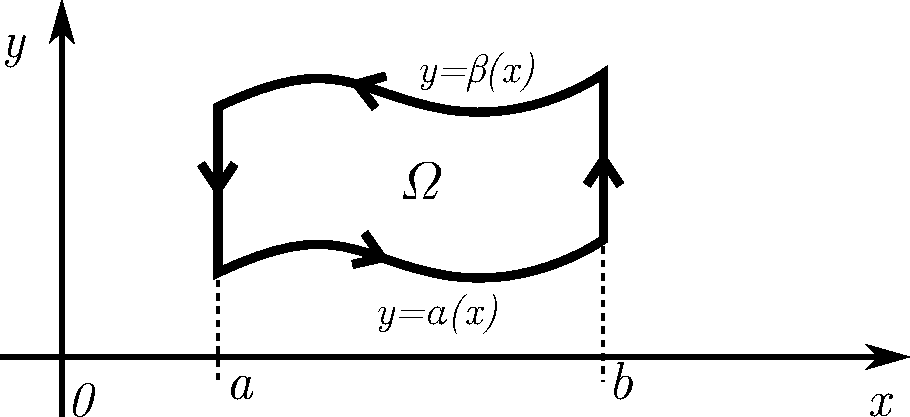
\includegraphics[width=0.8\textwidth]{nor_dom.pdf}
	\caption{Dominio normale per la dimostrazione delle formule di Green}
	\label{nor_dom}
\end{figure}
\noindent
si ha
\[
	\int_{\Omega} \partial_y f (x,y) dx dy=
	\int_a^b \int_{\alpha(x)}^{\beta(x)}
	\partial_y f (x,y) dx dy=
	\int_a^b \left[
		f(x,y)
	\right]_{y=\alpha(x)}^{y=\beta(x)}dx
\]
\[
	= \int_a^b \left[
	f(x,\beta (x)) - f(x, \alpha(x))
	\right] dx
\]
Per il tratto di frontiera
\[
	\left\{ 
	\begin{array}{ll}
		x=x & x \in [a,b] \\
		y= \alpha(x)
	\end{array}
	\right.
\]
si ha
\[
	{\bf T}= \frac{1}{\sqrt{1+ (\alpha ' )^2}}(1,\alpha ')
\]
\[
	ds= \sqrt{1+ (\alpha ' )^2} dx
\]
quindi, dato che il dominio \`e normale,
\[
	{\bf T} \cdot \uvi ds= dx
\]
perci\`o
\[
	\int \limits_{\gamma_{[a,b]}} f(x,y)\uvi \cdot {\bf T} ds
	= \int_a^b f(x, \alpha(x)) dx
\]
Per il tratto orientato in senso contrario
\[
	\left\{ 
	\begin{array}{ll}
		x=x & x \in [b,a] \\
		y= \beta(x)
	\end{array}
	\right.
\]
si ha
\[
	{\bf T}= - \frac{1}{\sqrt{1+ (\beta ' )^2}}(1,\beta ')
\]
\[
	ds= \sqrt{1+ (\beta ' )^2} dx
\]
quindi, dato nuovamente il dominio normale,
\[
	{\bf T} \cdot \uvi ds= -dx
\]
perci\`o
\[
	\int \limits_{\gamma_{[b,a]}} f(x,y)\uvi \cdot {\bf T} ds
	= \int_b^a f(x, \beta(x)) dx
	= -\int_a^b f(x, \beta(x)) dx
\]
Nei due tratti verticali si ha ${\bf T} = \pm \uvj$, 
quindi ${\bf T} \cdot \uvi = 0$.\\
Per concludere
\[
	\int_{\gamma} f(x,y)\uvi \cdot {\bf T} ds = 
	\int_a^b f(x, \alpha(x)) dx
	- \int_a^b f(x, \beta(x)) dx=
\]
\[
	- \int_a^b \left[ f(x, \beta(x)) -f(x, \alpha(x)) \right] dx
\]
e quindi
\[
	\int_{\gamma} f(x,y)\uvi \cdot {\bf T} ds =
	- \int_{\Omega} \partial_y f (x,y) dx dy=
\]
